\documentclass{article}
\usepackage{graphicx} % Required for inserting images
\usepackage{natbib}
\bibliographystyle{plain}

\title{Distributed Database using Vitess}
\author{Paul Wochnowski, Thomas Adler}
\date{December 2025}

\begin{document}

\maketitle

\begin{abstract}
This project presents the design and implementation of a distributed data center using Vitess, a database clustering middleware for MySQL. We architected a distributed database system capable of handling heterogeneous data where structured entities are partitioned by geographic region, content category, and temporal dimensions. The system features a transparent routing layer through an optimised distributed query processor, a high-throughput bulk loading mechanism, multimedia storage integration, and reliable replication topology with automated failover for all components of the system. On top of the database backend our system makes use of an in-memory caching mechanism, a comprehensive observability stack using Prometheus and Grafana with alerting capabilities, and a web-based frontend for interactive data exploration and querying. The resulting implementation demonstrates a highly available, elastic system capable of dynamic horizontal scaling and efficient cross-shard query processing, effectively satisfying the complex requirements of a distributed production environment.
\end{abstract}

\section{Introduction}

\subsection{Background and Motivation}
Modern software applications increasingly rely on data-intensive processes where storage requirements and query throughput exceed the capabilities of single-node database systems. Consequently, distributed database management systems (DDBMS) have become essential infrastructure. By leveraging horizontal scaling, these systems distribute data across multiple nodes to ensure performance and system availability. Beyond scalability, they enforce paradigms such as fault tolerance through data replication and location transparency, allowing applications to interact with physically fragmented data as a single logical entity.

The primary motivation for this work is to understand existing implementations for these distributed mechanisms, specifically regarding data fragmentation, replication, and fault tolerance. 

\subsection{Problem Definition}
The core objective is to design and implement a distributed data center capable of managing a hybrid dataset comprising five structured relational tables (User, Article, Read, Be-Read, Popular-Rank) alongside unstructured multimedia data (text, images, video). The system must enforce strict, attribute-based fragmentation and replication rules for the relational tables.

\subsubsection{Architecture Overview}
The target architecture consists of two geographically distributed sites (DBMS1 and DBMS2), each containing multiple database instances with associated caching layers and application servers. A shared Hadoop HDFS cluster provides distributed storage for multimedia content (article text, images, and videos). Figure~\ref{fig:architecture-overview} illustrates this high-level topology.

\begin{figure}[htbp]
  \centering
  \includegraphics[width=0.9\textwidth]{figures/architecture-overview.png}
  \caption{High-level architecture showing two data centers with application servers, caching layers, database instances (including standby replicas), and shared HDFS storage.}
  \label{fig:architecture-overview}
\end{figure}

\subsubsection{Fragmentation Requirements}
All five relations must be horizontally fragmented based on specific attribute values. Table~\ref{tab:fragmentation} summarizes the fragmentation and allocation rules.

\begin{table}[htbp]
\centering
\caption{Fragmentation and allocation rules for all relations}
\label{tab:fragmentation}
\begin{tabular}{|l|l|l|l|}
\hline
\textbf{Relation} & \textbf{Fragment Attribute} & \textbf{DBMS1} & \textbf{DBMS2} \\
\hline
User & \texttt{region} & Beijing & Hong Kong \\
\hline
Article & \texttt{category} & science & science, technology \\
\hline
Read & \texttt{region} & Beijing & Hong Kong \\
\hline
Be-Read & \texttt{category} & science & science, technology \\
\hline
Popular-Rank & \texttt{temporalGranularity} & daily & weekly, monthly \\
\hline
\end{tabular}
\end{table}

Notably, the ``science'' fragments of the Article and Be-Read relations are \emph{replicated} at both sites to ensure high availability for frequently accessed scientific content, while all other fragments reside exclusively at one site.

\subsubsection{Functional Requirements}
Beyond the storage and fragmentation requirements, the system must provide:
\begin{enumerate}
    \item \textbf{Bulk data loading} with automatic partition routing and replica consideration
    \item \textbf{Distributed CRUD operations} with efficient execution of inserts, updates, and cross-shard queries
    \item \textbf{System monitoring} including workload metrics, data distribution, and server status
    \item \textbf{Fault tolerance} through hot/cold standby mechanisms with automated failover
    \item \textbf{Cluster elasticity} supporting dynamic addition and removal of database nodes
    \item \textbf{Data migration} capabilities between data centers
\end{enumerate}

\subsection{Possible Distributed Solutions}
Implementing a custom distributed database from scratch was neither feasible nor sensible given the project timeline and complexity involved. Instead, we evaluated existing middleware solutions that operate between the application and database layers, managing sharding, replication, and query routing while presenting a unified logical database to the application.

The specific requirements of this project---particularly the need to fragment relations based on semantic attribute values and maintain fine-grained control over fragment placement and selective replication---significantly constrained our options.

\subsubsection{Citus}
Citus~\citep{citus} is a prominent extension that transforms PostgreSQL into a distributed database. While it effectively scales PostgreSQL workloads horizontally, it operates as an extension tightly coupled to the database engine rather than as independent middleware, offering less separation between the routing and storage layers.

More critically, Citus employs hash-based or range-based sharding strategies that cannot dynamically control fragment placement based on semantic rules. It is not possible to specify that rows with \texttt{region='Beijing'} should reside on one node while \texttt{region='HongKong'} rows reside on another. Furthermore, Citus does not support conditional replication where only specific attribute values (e.g., \texttt{category='science'}) are replicated across sites.

\subsubsection{CockroachDB}
CockroachDB~\citep{cockroachdb} is a distributed SQL database offering robust fault tolerance and strong consistency guarantees. However, it employs automatic load balancing and replica placement algorithms that prioritize even data distribution across nodes.

While this approach simplifies operations, it fundamentally conflicts with our requirement to \emph{design} the data distribution rather than allowing the system to determine it automatically. CockroachDB does not support conditional replication based on column values, making it impossible to replicate only ``science'' articles to both sites while keeping ``technology'' articles on a single site.

\subsubsection{Vitess}
We selected Vitess~\citep{vitess} as the core technology for our distributed database system. Vitess is an open-source database clustering system that provides a middleware layer for horizontally scaling MySQL. Originally developed at YouTube to manage massive database workloads serving billions of daily queries, it is now a Cloud Native Computing Foundation (CNCF) graduated project used in production by organizations including Slack, Square, and GitHub.

Vitess was uniquely suited to our requirements for several reasons:
\begin{itemize}
    \item \textbf{Custom Vindexes}: Vitess supports pluggable sharding functions (vindexes) including the \texttt{region\_json} type, which maps attribute values to specific shards via configurable JSON mappings.
    \item \textbf{Explicit Shard Placement}: Each shard can be assigned to specific cells (data centers), enabling precise control over data locality.
    \item \textbf{Cross-Site Replication}: Vitess supports replica tablets in different sites, allowing selective replication of specific shards across sites.
    \item \textbf{Transparent Query Routing}: The VTGate proxy layer parses queries and routes them to appropriate shards, supporting both targeted queries and scatter-gather operations for cross-shard joins.
    \item \textbf{Operational Maturity}: Built-in support for automated failover (VTOrc), integration with prometheus, and backup/restore operations.
\end{itemize}

\section{System Design}

Figure~\ref{fig:system-architecture} presents the complete system architecture, illustrating the data path from client applications through the distributed database layer, alongside the control plane components and supporting infrastructure. The following subsections describe each layer in detail.

\begin{figure}[htbp]
  \centering
  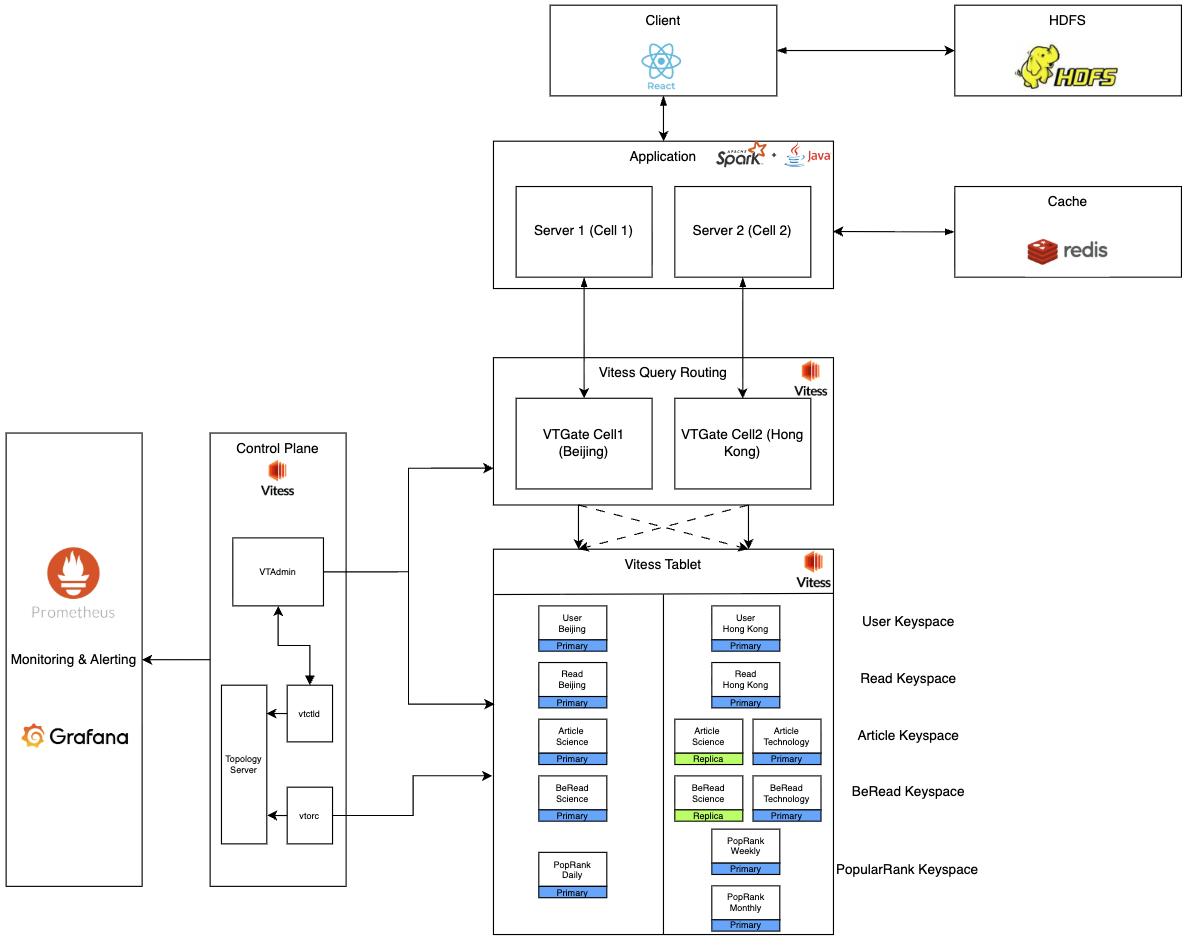
\includegraphics[width=\textwidth]{figures/system-architecture.png}
  \caption{System architecture showing the data path (Client $\rightarrow$ Application $\rightarrow$ VTGate $\rightarrow$ VTTablet), the Vitess control plane (Topology Server, VTCtld, VTOrc), and supporting infrastructure (Redis cache, HDFS storage, Prometheus/Grafana monitoring).}
  \label{fig:system-architecture}
\end{figure}

\subsection{Vitess Architecture}
The Vitess platform consists of several server processes that can be categorized into the \emph{data path}---responsible for query routing and execution---and the \emph{control plane}---responsible for cluster management and coordination.

\subsubsection{Data Path Components}

A \textbf{keyspace} is a logical database that maps to one or more MySQL databases. In our implementation, each of the five relations (User, Article, Read, Be-Read, Popular-Rank) is represented as a separate keyspace. A keyspace can be \emph{sharded}, meaning its data is partitioned across multiple databases, or \emph{unsharded} if it resides in a single database.

A \textbf{shard} is a horizontal partition within a keyspace. Each shard contains a subset of the keyspace's data and typically consists of one MySQL primary and potentially many MySQL replicas. These MySQL instances within a shard are referred to as \textbf{tablets}. A tablet is designated a type: \texttt{PRIMARY} for the authoritative copy handling writes, or \texttt{REPLICA} for read-only copies that replicate from the primary.

Queries are routed to tablets via a \textbf{VTGate} server. VTGate is a stateless proxy that speaks the MySQL protocol, allowing applications to connect as if communicating with a standard MySQL server. It parses incoming queries, consults the sharding schema---which encodes fragmentation rules, shard locations, and routing logic---to determine which shards contain the relevant data, routes queries to the appropriate tablets, and aggregates results from multiple shards when necessary.

\subsubsection{Control Plane Components}

The \textbf{Topology Server}, implemented using Consul in our deployment, is a distributed key-value store that maintains cluster metadata including keyspace definitions, shard assignments, and tablet locations. It enables VTGates and tablets to discover each other and coordinate cluster state.

\textbf{VTOrc} (Vitess Orchestrator) monitors tablet health and performs automated failover when a primary becomes unavailable, promoting a replica to primary without manual intervention. Its operation is detailed in Section~\ref{sec:fault-tolerance}.

\textbf{VTCtld} and \textbf{VTAdmin} provide administrative interfaces for cluster management. VTCtld exposes a gRPC API for operations such as schema changes and shard management, while VTAdmin offers a web-based dashboard for cluster visualization.

\subsubsection{Multi-Cell Topology}

A \textbf{cell} is a group of servers that are geographically colocated and share regional availability, typically corresponding to a data center or availability zone. Each cell contains its own VTGate pool and a set of tablets.

Tablets are assigned to a specific cell, but tablets belonging to the same shard can be placed in different cells. This enables geographic distribution of replicas, allowing read traffic to be served locally while maintaining data durability across regions.

The topology service is split into a \emph{global topology}, which stores cluster-wide metadata such as keyspace and shard definitions and is distributed across cells for fault tolerance, and \emph{local topologies} within each cell containing cell-specific tablet information. VTGates and tablets read primarily from their local topology for efficiency.

VTGate prefers tablets in its cell when routing read queries, minimizing network latency. Write queries are always routed to the shard's primary tablet regardless of its cell location.

\subsection{Storage}

The sharding configuration for each keyspace is defined in a \textbf{VSchema} (Vitess Schema), which specifies fragmentation rules, vindex declarations, and table-to-vindex bindings. The VSchema is stored in the global topology and distributed to all VTGate instances, enabling consistent query routing across the cluster.

\subsubsection{Fragmentation}

Vitess implements horizontal fragmentation through \textbf{Vindexes} (virtual indexes). Each sharded table declares a \textbf{Primary Vindex} that determines shard placement at insert time. The Primary Vindex computes a keyspace ID from column values---unlike traditional sharding keys, this value is not stored in a physical column but computed on-demand. Vitess supports pluggable vindex types, allowing the sharding strategy to be customized per table.

For our attribute-based fragmentation requirements, we use the \texttt{region\_json} vindex type, which maps column values to shards via a configurable JSON document. This enables semantic partitioning: the User and Read tables shard by \texttt{region}, Article and Be-Read by \texttt{category}, and Popular-Rank by \texttt{temporalGranularity}, directly satisfying the fragmentation rules in Table~\ref{tab:fragmentation}.

A limitation of attribute-based sharding is that queries on non-sharding columns (e.g., retrieving a user by \texttt{uid} rather than \texttt{region}) would require a scatter query to all shards. Vitess addresses this with \textbf{Lookup Vindexes}---secondary vindexes backed by a lookup table that maps column values to their containing shard. We define lookup vindexes for primary key columns (\texttt{uid}, \texttt{aid}, etc.), allowing VTGate to resolve the target shard with a single lookup. These lookup tables are automatically maintained by Vitess during insert and delete operations.

\subsubsection{Allocation}

Each shard is assigned to a cell by placing its tablets within that cell's infrastructure. For shards that reside exclusively in one site (e.g., Beijing users, technology articles, weekly/monthly rankings), a single PRIMARY tablet is deployed in the corresponding cell. For the science category shards, which require cross-site availability, we deploy a replica tablet in each cell and allow VTOrc to promote one as PRIMARY. This ensures that both cells can serve reads locally, while VTOrc manages failover automatically if the primary becomes unavailable.

\subsection{Query Processing}

VTGate is the stateless proxy responsible for query planning and routing. It parses incoming SQL, builds an execution plan that determines which shards to query, and aggregates results when necessary—presenting the illusion of a single logical database to the application.

\subsubsection{Planning and Routing}

VTGate builds execution plans as operator trees, where leaf nodes called \emph{routes} send queries to one or more shards. The planner's goal is to push as much work as possible down to MySQL, minimizing processing at the VTGate layer.

When a query includes the sharding column in its WHERE clause, VTGate uses the vindex to route directly to the appropriate shard. Without a sharding column, VTGate performs a \emph{scatter} query, sending the request to all shards and merging results. For cross-shard joins, VTGate may split the query, fetch data from multiple shards, and join the results locally. VTGate also rewrites queries to maintain the single-database illusion despite connection pooling. 

\subsubsection{Transactions}

Vitess supports three transaction modes: \emph{Single} (disallows multi-shard transactions), \emph{Multi} (best-effort commits across shards), and \emph{TwoPC} (atomic cross-shard commits via two-phase commit). Single-shard transactions remain fully ACID, but Multi mode may result in partial commits if a failure occurs mid-transaction. TwoPC provides distributed atomicity at the cost of approximately 50\% higher write latency. Since strict cross-shard atomicity is not critical for our use case, we use the default Multi mode.

\subsection{App Server}

The application server layer mediates between client applications and the distributed database, providing a unified API for data access while integrating caching and multimedia content resolution.

\subsubsection{HTTP Server}

The server is implemented in Java using the Spark micro-framework, a lightweight embedded HTTP server well-suited for RESTful services. Critically, the architecture deploys a separate application server instance in each data center, with each instance connecting to its co-located VTGate via the standard MySQL protocol. This stateless, distributed design avoids a centralized bottleneck where all client requests would otherwise funnel through a single server, and allows clients to interact with their geographically nearest endpoint for reduced latency.

The API exposes RESTful endpoints for all five entities, supporting standard CRUD operations with Protocol Buffers for efficient binary serialization. Query endpoints accept RSQL filter expressions, which are parsed and translated to SQL WHERE clauses, enabling flexible client-side filtering, sorting, and pagination.

\subsubsection{In-memory Cache}

Redis, an in-memory key-value store, provides a caching layer to reduce database load for frequently accessed data. The cache is used for isolated GET-by-ID requests for articles; on cache miss, the server fetches from the database and populates the cache, while updates and deletes trigger cache invalidation to maintain consistency.

\subsubsection{Multimedia}

Multimedia content (article text, images, and videos) is stored in a Hadoop HDFS cluster comprising one NameNode and two DataNodes. Rather than streaming files through the application server, the intended workflow returns WebHDFS download URLs to the client, which then fetches the content directly from HDFS. This approach offloads bandwidth from the application server and avoids it becoming a bottleneck for large file transfers.

\subsection{Fault Tolerance}

Vitess provides multiple layers of fault tolerance across the data and control planes. VTGate continuously monitors tablet health and automatically detects when a tablet becomes unavailable, routing queries to healthy replicas without application intervention. If a primary tablet fails, VTOrc orchestrates automated failover by electing a new primary from the available replicas---this promotion can occur across cell boundaries if necessary, ensuring continuity even when an entire data center becomes unreachable.

Most Vitess components---including VTGate, VTTablet, and VTCtld---are stateless and can be restarted or replaced without data loss. The topology service is the sole stateful component in the control plane; it maintains cluster metadata using Raft consensus to achieve majority agreement among nodes. To survive a complete cell failure, the global topology service should be deployed with nodes distributed across multiple cells, ensuring that a quorum can be maintained even if one cell goes offline.

To prevent data loss during failover, Vitess leverages MySQL's semi-synchronous replication: a transaction is not acknowledged as committed until at least one replica has received and persisted the change. This ensures that if a primary fails, the promoted replica contains all committed transactions, avoiding the data loss scenarios possible with purely asynchronous replication.

\section{System Capability}

\subsection{Bulk Data Loading}

The system supports bulk loading of the User, Article, and Read tables with 10,000, 10,000, and 50,000 records respectively. A Python script connects to VTGate and issues batched multi-row INSERT statements, with VTGate automatically routing each record to the appropriate shard based on the configured vindexes. The script disables constraint checks (\texttt{unique\_checks=0}, \texttt{foreign\_key\_checks=0}) during loading to reduce per-row overhead.

To maximize throughput, a wrapper script temporarily disables semi-synchronous replication on all primary tablets before invoking the bulk insert. This eliminates the per-commit latency of waiting for replica acknowledgment, allowing writes to complete immediately. After the bulk load finishes, the wrapper re-enables semi-sync to restore durability guarantees for normal operations.

% TODO: Add timing results
% - Total load time: X seconds
% - Throughput: X records/second
% - Comparison with/without semi-sync disabled

\subsection{CRUD Operations}

All CRUD operations are issued against VTGate, which routes queries to the appropriate shard based on the vindex. When the sharding column appears in the WHERE clause, VTGate targets the specific shard; otherwise, it performs a scatter query across all shards. The application server exposes RESTful endpoints using Protocol Buffers for efficient binary serialization.

\subsubsection{Insert}

Standard MySQL auto-increment does not work across shards, as each shard would generate conflicting IDs independently. Vitess addresses this with \emph{sequences}---unsharded single-row tables that generate monotonically increasing IDs. The VSchema binds a table's ID column to its sequence, so INSERT statements transparently fetch the next ID before routing the row to the appropriate shard.

\subsubsection{Read}

Read requests for individual records by ID first check the Redis cache; on cache miss, the record is fetched from the database and cached for subsequent requests. The API supports RSQL filter expressions, which are parsed and translated to SQL WHERE clauses for flexible client-side querying.

\subsubsection{Update}

Updates follow the same routing logic. On successful update, the corresponding cache entry is invalidated to ensure consistency.

\subsubsection{Delete}

Deletes similarly invalidate the cache entry for the affected record.

\subsection{Cross-Shard Joins}

The UserRead view requires joining the User and Read tables, which reside in separate keyspaces sharded by region. VTGate handles this cross-keyspace join transparently, and its query optimizer pushes filter predicates down to individual shards to minimize data transfer. For example, filtering UserRead by region halves the query time compared to an unfiltered query, as only the relevant shard is queried rather than scattering across all shards.

\subsection{System Monitoring and Alerts}

\subsubsection{Metrics Collection}

Metrics are collected from two sources. Container-level metrics (CPU, memory, network I/O) are gathered via cAdvisor, which exposes Docker container statistics. Vitess components (VTGate, VTTablet) expose application-level metrics---including query counts, latency histograms, and replication lag---on their \texttt{/metrics} endpoint in Prometheus format. Prometheus scrapes both sources and applies relabeling rules to extract structured labels (keyspace, shard, role) from container names.

\subsubsection{Dashboards}

Grafana connects to Prometheus and provides real-time visualization of cluster health, query performance, and resource utilization across all tablets and gateways.

% TODO: Add figure showing Grafana dashboard

\subsubsection{Alerting}

Prometheus evaluates alerting rules and forwards triggered alerts to Alertmanager, which handles deduplication, grouping, and notification routing. Example rules include high CPU usage on tablets and replication lag thresholds. Alertmanager can be configured to deliver notifications via email, Slack, or other channels.

\subsection{Fault Tolerance and Cluster Elasticity}

Vitess handles hot standby and cluster expansion through the same mechanism: adding replica tablets. New tablets restore from the most recent backup and replay the binlog to catch up on subsequent changes before being marked operational and joining the serving pool. VTGate automatically discovers new tablets, and VTOrc monitors tablet health to promote a replica to primary if the current primary fails.

\subsubsection{Hot Standby}

A hot standby is simply a replica tablet. To demonstrate cross-cell failover, we deploy the replica in a separate cell from the primary. When the primary becomes unavailable, VTOrc automatically promotes the replica, and VTGate reroutes traffic without application intervention.

\subsubsection{Adding Nodes}

Adding a new tablet follows the same process: start a VTTablet instance pointing to the appropriate shard, and it initializes from backup. Once caught up, VTGate begins routing queries to it.

\subsubsection{Removing Nodes}

To remove a tablet, it is drained of traffic and deleted from the topology. VTGate stops routing to the removed tablet immediately.

\subsection{Data Migration}

To migrate data between data centers, we create a full clone of the source cluster via backup and restore. A script first triggers backups of all shards in DC1, then spawns DC2 as an independent Vitess cluster with its own topology service. DC2 tablets are configured to restore from the shared backup volume on startup, initializing with a complete copy of DC1's data. Once restored, DC2 operates independently with its own VTGates and can serve traffic for the migrated data.


\section{Conclusion}

\subsection{Future Work}
Future iterations would benefit from migrating the deployment orchestration from Docker Compose to Kubernetes using the Vitess Operator, which would enable cloud-native auto-scaling capabilities. Furthermore, implementing SSL/TLS encryption for inter-component communication and authentication for the VTGate interface would enhance production security. Finally, integrating a dedicated OLAP engine to handle analytical workloads for the \textit{Popular-Rank} table could further optimize the performance of the transactional cluster.

\subsection{Summary}
In this project, we successfully designed and implemented a distributed data center using Vitess that manages five relational tables alongside unstructured multimedia content accessed via HDFS. The system enforces strict attribute-based fragmentation strategies—including region-based, category-based, and temporal-based partitioning—supported by a topology featuring Primary tablets for all shards and targeted cross-cell Replicas for high-demand "Science" categories to ensure availability. We integrated high-throughput bulk loading, Redis caching for read optimization, and a React-based frontend for location-aware client interaction. By incorporating Prometheus and Grafana monitoring with VTOrc-managed automated failover, the system achieves fault tolerance and location transparency while supporting dynamic cluster operations. The implementation demonstrates a practical, scalable solution to the challenges of distributed data management in a multi-cell environment.

\subsection*{Work Allocation}
PW was responsible for the core distributed architecture, including all the Vitess-related implementation and the frontend, fragmentation logic, and the integration of Hadoop HDFS and Redis. TA implemented Prometheus and Grafana for monitoring and alerting, while also writing the first draft of the system manual and final research report. Both reviewed it and wrote the final versions.

\bibliography{references}

\end{document}
